
%%%%%%%%%%%%%%%%%%%%%%%%%%%%%%%%%%%%%%%%%
% University/School Laboratory Report
% LaTeX Template
% Version 3.0 (4/2/13)
%
% This template has been downloaded from:
% http://www.LaTeXTemplates.com
%
% Original author:
% Linux and Unix Users Group at Virginia Tech Wiki 
% (https://vtluug.org/wiki/Example_LaTeX_chem_lab_report)
%
% License:
% CC BY-NC-SA 3.0 (http://creativecommons.org/licenses/by-nc-sa/3.0/)
%
%%%%%%%%%%%%%%%%%%%%%%%%%%%%%%%%%%%%%%%%%

%----------------------------------------------------------------------------------------
%	PACKAGES AND DOCUMENT CONFIGURATIONS
%----------------------------------------------------------------------------------------



\documentclass[11pt,a4paper,polish]{article}
\usepackage[T1]{fontenc}
\usepackage[utf8]{inputenc}
\usepackage{babel}
\usepackage{blindtext}
\usepackage{graphicx} 
\usepackage{url}

\linespread{1.3} %interlinia
\addtolength{\textwidth}{3cm}
\addtolength{\hoffset}{-1.5cm}
\addtolength{\textheight}{3cm}
\addtolength{\voffset}{-1.5cm}

\usepackage{graphicx} % Required for the inclusion of images


%----------------------------------------------------------------------------------------
%	DOCUMENT INFORMATION
%----------------------------------------------------------------------------------------

\title{Algorytmy rotorowe - symulacja\\
Zaawansowane metody kryptografii i ochrony informacji 
}
\date{13 czerwca, 2013}
\author{Lukasz Sedek\\ Politechnika Warszawska
        \and Marcin Toczko\\ Politechnika Warszawska
        \and \{L.Sedek, M.Toczko\}@stud.elka.pw.edu.pl\\
        prowadzący: mgr inż. Marcin Tunia\\
        semestr: 2013 LATO}
        
\begin{document}


\maketitle % Insert the title, author and date
\newpage

%----------------------------------------------------------------------------------------
%	WPROWADZENIE
%----------------------------------------------------------------------------------------

\section{Wprowadzenie}

Niniejsza praca jest projektem na przedmiot Metody Kryptografii i Ochrony
Informacji. Opracowane w niej zostało działanie algorytów rotracyjnych na
podstawie symulacji szyfratora Enigma.

 
%----------------------------------------------------------------------------------------
%	SECTION 2
%----------------------------------------------------------------------------------------

\section{Opracowanie teoretyczne}

Mechanizm rotacyjny wykorzystywany jest przez szyfry strumieniowe. Zasada
działania szyfrów strumieniowych opiera na szyfrowaniu jawnego tekstu ze 
znanego alfabetu (uporządkowanego zbioru możliwych danych wejściowych) i klucza
bieżącego. Kluczem bieżącym może być dowolna fraza o długości nie mniejszej
od długości tekstu szyfrowanego (jawnego)[1]. Jednak użycie tekstu w roli klucza bieżącego ( fragmentu książki ) stwarza możliwość odczytania wiadomości
wykorzystując redundancję języka. Zalecane jest stosowanie losowego ciągu nie
przenoszącego żadnej logicznej informacji, zarazem dany ciąg losowy powinien
być wykorzystany tylko jeden raz. Wtórne użycie danego ciągu, zwiększa prawdopodobieństwa odczytania wiadomości.
Zilustrowaną zasadę działania rotorów przedstawiono na rysunku 1. Podstawą
działania są niezależnie obracające się cylinry, które przenoszą syngał elektryczny. Rysunek jest przedstawia realizację Enigmy. Każdy cylinder jest wyposażony
w 26 styków wejściowych i 26 wyjściowych oraz wewnętrzne przewody łączące
każdy styk wejściowy z odpowiadającym mu wyjściowym. Złożoność, jak i siła
szyfrowania tkwi w liczbie cylindrów i liczbie permutacji jakie mogą nastąpić.
Proces odwrotny do szyfrowania jest możliwy jedynie , gdy układ cylindrów
po stronie nadawczej oraz odbiorczej jest taki sam. Kluczem algorytmicznym
jest identyczne ustawienie początkowe walców w maszynach. Podczas II wojny światowej Enigma była wykorzystywana jako główne narzędzie szyfrujące w
rękach III Rzeszy. Siła takiego rozwiązania polegała, na częstej zmianie kluczy
szyfrujących (klucze dzienne). Podstawą działania była operacja podstawienia,
wchodząca litera była zamian zgodnie z ustawieniem stykami w danym rotorze
na inną. Złożoność systemu polegała na wielokrotnym użyciu operacji podstawienia. Po każdorazowym naciśnięciu klawisza następowała zmiana ustawień
rotorów.
Zaletą takich algorytmów jest duży okres powtarzalności klucza. Dla szyfratora
z alfabetem 26 znakowym i liczbą cylindrów k, klucz zostanie powtórzony co
26k obrotów najwolniejszego cylindra[2].
\begin{figure}
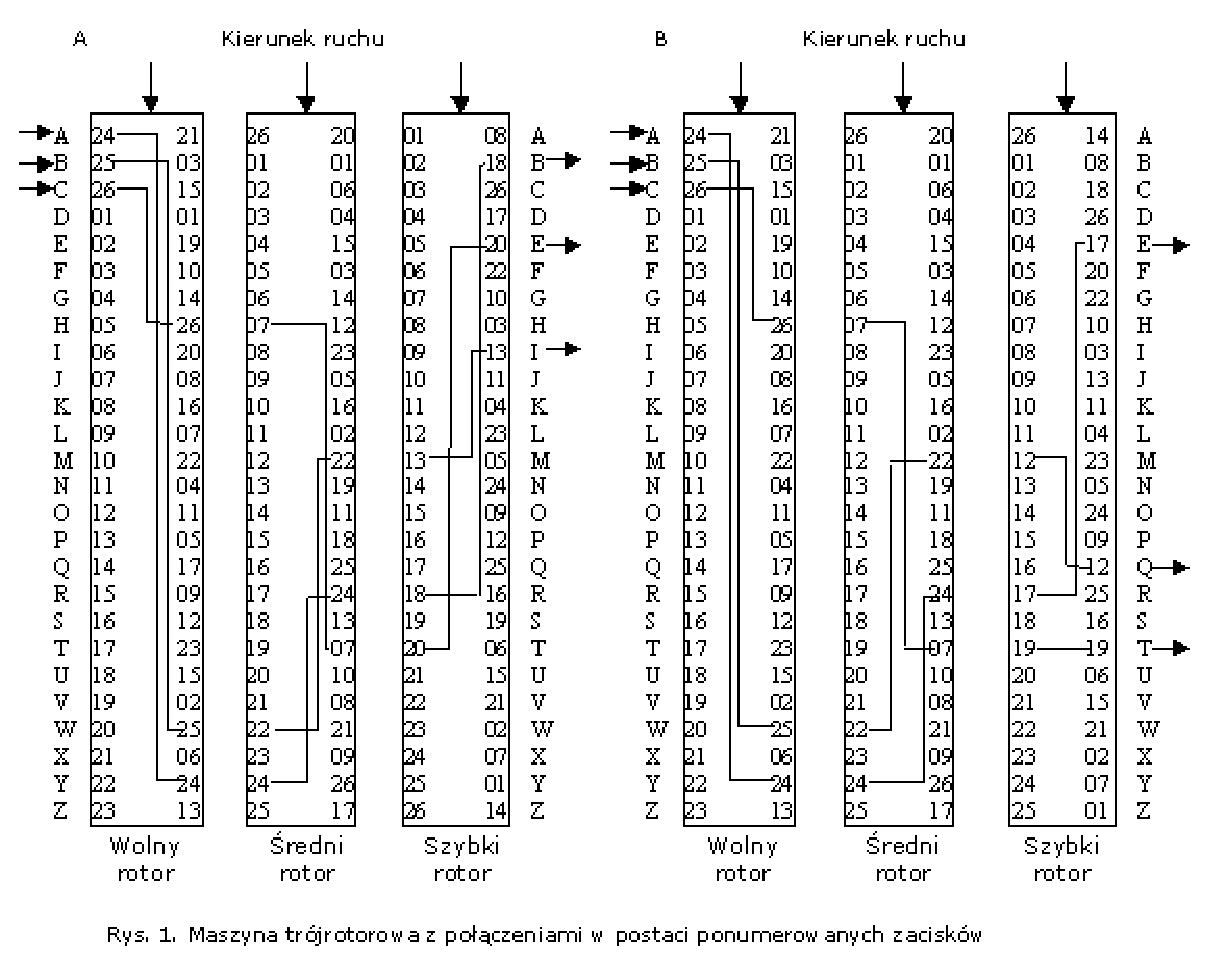
\includegraphics[scale=0.8]{rotors.eps}
\end{figure}

\newpage
%----------------------------------------------------------------------------------------
%	SECTION 3
%----------------------------------------------------------------------------------------

\section{Opis algorytmu}
\subsection{Dane wejściowe}
Przykładowy plik konfiguracyjny:
\begin{verbatim}
# PLIK KONFIGURACYJNY
rozmiar = 26
alphabet = ABCDEFGHIJKLMNOPQRSTUVWXYZ
reflector = YRUHQSLDPXNGOKMIEBFZCWVJAT
liczba_rotorow = 3
rotor0 = EKMFLGDQVZNTOWYHXUSPAIBRCJ
rotor0_start = Q
rotor0_turn = Q
rotor1 = AJDKSIRUXBLHWTMCQGZNPYFVOE
rotor1_start = E
rotor1_turn = E
rotor2 = BDFHJLCPRTXVZNYEIWGAKMUSQO
rotor2_start = V
rotor2_turn = V

\end{verbatim}
%----------------------------------------------------------------------------------------
%	SECTION 4
%----------------------------------------------------------------------------------------

\section{zastosowania praktyczne implementowanego zagadnienia}
W dzisiejszych czasach stosowanie algorytmów rotorowych jest rozwiązaniem
historycznym i z dostępnych źródeł trudno znaleźć przykłady zastosowań w
istniejących szyfratorach. Natomiast, znaczenie historyczne Enigmy jest tak
duże, że stanowi cenny materiał dydaktyczny dla potrzeb nauki kryptografii
i kryptoanalizy\cite{4640685,Hodges}.

%----------------------------------------------------------------------------------------
%	SECTION 5
%----------------------------------------------------------------------------------------

\section{Instrukcja użytkowania programu}
Aplikacja została napisana w języku Java. Szkielet programu został
zautomatyzowany przy pomocy narzędzia maven i wzorca programowania MVC. Do
stworzenia GUI zastosowane zostały domyślne biblioteki graficzne Swing
(wbudowane w język Java).
\subsection{Wymagania}
\begin{itemize}
  \item Java JDK wersja 1.7 . Używane są elementy wersji 7 np. JList<E>.
  \item Maven wersja co najmniej 2.1
  \item Narzędzie do repozytoriun GIT.
\end{itemize} 
\subsection{Instalacja}
Instalacja została zautomatyzowana. Aby ściągnąć repozytorium na maszynę
lokalną, niezbędne jest zsynchronizowanie się z repozytorium, które jest
dostępne pod adresem\\
\textit{git@github.com:lukaszsedek/mkoi.git}\cite{Git}
. Instalacja przebiega zgodnie z
zasadami budowania aplikacji przy użyciu narzędzia maven. Aby stworzyć
uruchamialny plik \textit{jar}, należy wydać polecenie w katalogu
\textit{mkoi}
\begin{verbatim}
# mvn clear install
\end{verbatim}
Następnie należy upewnić się czy został stworzony katalog \textit{target}.
\subsection{Uruchomienie}
Program nie zawiera żadnych dodatkowych plików wymaganych do załączenia przy
uruchamianiu, więc należy wpisać:
\begin{verbatim}
# java -jar target/mkoi-0.2.jar
\end{verbatim}
Na ekranie pojawi się okno jak na poniższym rysunku. Lewa strona do służy do
wprowadzania bieżącego tekstu - szyfrowanego tekstu. Natomiast prawe okno służy
do wyświetlania zaszyfrowanego tekstu z lewej strony. Środek stanowi element
graficzny przedstawiający aktualne położenie rotorów. Pierwszą czynnością jaką
użytkownik powinien wykonać, to załadowanie pliku konfiguracyjnego. Następny
krok to wpisywanie tekstu do szyfrowania. Szyfrowanie odbywa się `w locie`.
\newpage
\begin{figure}
\includegraphics[scale=0.43]{mkoi.eps}
\end{figure}


%----------------------------------------------------------------------------------------
%	Testy
%----------------------------------------------------------------------------------------

\section{Testy}
Zostały wykonane testy jedynie funkcjonalne i jednostkowe. Testowanie
jednostkowe opierało się na debugowaniu stanów rotorów w programie (tzw.
\textit{grey-box testing}).\\
Testy funkcjonalne polegały na sprawdzaniu wartości wyjściowych przy znanych
wartościach wejściowych(pobrane z \cite{wiki, Hamer}).
Dane te to ustawienia początkowe rotorów, reflektora oraz przesunięcia. Wartości
te podawane były w pliku konfiguracyjnym i manualnie testowane. Wyniki
porównywaliśmy z symulatorem Enimgy\cite{enigmatut}.

%----------------------------------------------------------------------------------------
%	BIBLIOGRAPHY
%----------------------------------------------------------------------------------------

\bibliographystyle{unsrt}

\bibliography{bib}

%----------------------------------------------------------------------------------------


\end{document}